%%%%%%%%%%%%%%%%%%%%%%%%%%%%%%%%%%%%%%%%%%%%%%%%%%%%%%
% A template for Wiley article submissions.
% Developed by Overleaf. 
%
% Please note that whilst this template provides a 
% preview of the typeset manuscript for submission, it 
% will not necessarily be the final publication layout.
%
% Usage notes:
% The "blind" option will make anonymous all author, affiliation, correspondence and funding information.
% Use "num-refs" option for numerical citation and references style.
% Use "alpha-refs" option for author-year citation and references style.

% MRM style
\documentclass[num-refs]{wiley-article}
% \documentclass[blind,num-refs]{wiley-article}

% simple style
% \documentclass[num-refs]{mrm2plain}

% added for highlighting
\usepackage{soul}

% added for margin notes
\usepackage{marginnote}

\bibliographystyle{vancouver-authoryear}

% Add additional packages here if required
\usepackage{siunitx}

% Graphics. Always show the figures but float to the end
% code listing
%\usepackage[final]{subfig, listings}
%\usepackage[nofiglist]{endfloat}

\graphicspath{{./figures/}}

% Update article type if known
\papertype{Full paper}
% Include section in journal if known, otherwise delete
% \paperfield{Journal Section}

\title{Adaptive Baseline Fitting for $^{\textbf{1}}$H MR Spectroscopy Analysis}

% Use the \authfn to add symbols for additional footnotes and present addresses, if any. Usually start with 1 for notes about author contributions; then continuing with 2 etc if any author has a different present address.
\author[1]{Martin Wilson}

%\contrib[\authfn{1}]{Equally contributing authors.}

% Include full affiliation details for all authors
\affil[1]{Centre for Human Brain Health and School of Psychology, University of Birmingham, Birmingham, UK.}

\corraddress{Martin Wilson, Centre for Human Brain Health, University of Birmingham, Edgbaston, Birmingham, B15 2TT, United Kingdom.}

\corremail{wilsonmp@bham.ac.uk}

% \fundinginfo{Funder One, Funder One Department, Grant/Award Number: 123456, 123457 and 123458; Funder Two, Funder Two Department, Grant/Award Number: 123459}

% Include the name of the author that should appear in the running header
\runningauthor{Wilson}

% my macros
\newcommand{\proton}{\ensuremath{^1\mathrm{H}}}
\newcommand{\bzero}{\ensuremath{\mathrm{B}_0}}
\soulregister\bzero7 % needed for soul to work with this macro
\soulregister\ref7 % needed for soul to work with this macro
\soulregister\cite7 % needed for soul to work with this macro

% revision two highlighting
%\newcommand{\revtwo}[2]{\hl{#1}\marginnote{\hl{#2}}}
%\newcommand{\revtwonm}[1]{\hl{#1}} % no margin label

% uncomment next two lines to hide revision two highlighting
%\newcommand{\revtwo}[2]{#1}
%\newcommand{\revtwonm}[1]{#1}

\begin{document}

\maketitle

\begin{abstract}
\textbf{Purpose:} \\
\textbf{Methods:} \\
\textbf{Results:} \\
\textbf{Conclusion:} 
\keywords{XXXX}
\end{abstract}

Word count : XXXX

% MRM abstract max length is 250 words
% MRM note max length is 2800 words, 5 fig plus tables
% MRM full paper max length is 5000 words, 10 fig plus tables

\section{Introduction}
A number of key metabolites may be detected using \proton\ Magnetic Resonance Spectroscopy (MRS), providing a non-invasive measure of healthy and diseased brain tissue metabolism. Clinical applications include the assessment of brain tumors, metabolic disorders and neonatal encephalopathy~\cite{Oz2014,Lally2019} where the concentration of certain metabolites may inform disease diagnosis or predict patient outcome. Further applications for MRS are present in the neuroscience and psychiatry domains, with particular interest in the direct detection of neurotransmitter levels such as GABA and glutamate, which have been shown to be abnormal in Schizophrenia~\cite{Merritt2016} and modulate in response to tasks~\cite{Jelen2018,Chen2017}.

MRS scans are typically performed at short (30ms) or long (144ms) TE's, with short-TE scans being preferred due to reduced T2 relaxation and dephasing of multiplets resulting in improved metabolite detection sensitivity~\cite{Wilson2019}. However, short-TE scans are typically more susceptible to artifacts originating from insufficient water and scalp lipid suppression, in addition, broad signals from macromolecules also become enhanced~\cite{Cudalbu2012}. Residual water signals, lipid signals and macromolecules all have the potential to bias metabolite measurements due to spectral overlap and interference. Therefore, appropriate analysis methodology is particularly important to achieve the full benefit of conventional short-TE MRS.

Parametric fitting is currently the most widely used analysis method for MRS data, and typically incorporates a set of simulated metabolite signals --- known as a basis set. One of the main distinctions between analysis methods is their approach for mitigating metabolite estimation bias from broad signals not present in the basis set, usually referred to as ``baseline modeling''. One of the most popular baseline modeling methods incorporates a set of smooth spline functions into the fitting procedure, with additional smoothness imposed by penalizing greater baseline complexity. The LCModel~\cite{Provencher1993} and AQSES~\cite{Poullet2007} algorithms both use penalized spline baseline modeling, with analysis performed in the frequency-domain and time-domain respectively.

An alternative approach to baseline modeling exploits the rapid decay of baseline signals in the time-domain by omitting the preliminary data points during the fitting process, reducing their interference with the more slowly decaying metabolites. The QUEST~\cite{Ratiney2005} and TARQUIN~\cite{Wilson2011} methods both use this time-domain truncation approach. The FITT~\cite{Young1998} algorithm combines the wavelet transform with Lowess filtering in the frequency-domain to separate metabolite and baseline signals.

Control over the level of baseline flexibility (or smoothness) is a common and necessary requirement of each of the baseline modeling methods outlined above. For spline based approaches, the number of spline functions for a given frequency range and the smoothness penalty parameter control the baseline flexibility. For LCModel, the frequency spacing between the spline basis functions is dependent on data quality, and is set at maximum of 1.5 times the estimated full width at half maximum (FWHM) of the metabolite resonances or 0.1 ppm~\cite{Provencher1993}. Similarly, for the FITT algorithm a fixed Lowess filter smoothing value is used and wavelet coefficients with scales less than twice the FWHM are excluded from the baseline model to ensure smoothness~\cite{Young1998}. In the time-domain truncation approach baseline flexibility is primarily determined by the number of initial data points to be omitted from the fit evaluation. For QUEST and TARQUIN the number of truncated data points, and therefore degree of baseline flexibility, is set at a default value that may be adjusted by the user.

Automated methods to determine the correct degree of baseline flexibility are important for obtaining accurate metabolite levels independently of the analyst. Furthermore, the manual adjustment of baseline flexibility for each individual spectrum is impractical for MRSI studies --- where hundreds of spectra may be acquired in a single scan. Whilst LCModel provides automated adjustment of baseline flexibility, a growing number of analysts choose to manually override the default analysis settings by adjusting the spline spacing parameter (DKNTMN). The first reported use of this manual adjustment was to improve the modeling of macromolecular resonances in rat brain at 9.4 T~\cite{Pfeuffer1999}. More recently, this parameter has been adjusted to encourage flatter baselines~\cite{Deelchand2016,Terpstra2010,Marjanska2018}, suggesting the default LCModel baseline flexibility may not be optimal in some cases.

Finding the optimal degree of baseline flexibility is a crucial question in MRS analysis research, yet few studies have investigated this topic in detail. Using simulated data, Ratiney et al.\ demonstrated how the interference between metabolite and baseline signals was reduced by increasing the number of omitted data points, but this came at the cost of inflating errors due to noise~\cite{Ratiney2004}. More recently, Near et al.\ showed how the estimated baseline in LCModel can depend strongly on spectral SNR and metabolite FWHM, and that errors caused by baseline instability may dominate over errors from spectral noise in some cases~\cite{Near2013}. The influence of baseline flexibility has also been explored using experimentally acquired data, with a recent study demonstrating a 15\% difference in metabolite levels when comparing between a default and less flexible baseline model~\cite{Giapitzakis2019}. Baseline flexibility has also been shown to have a strong influence of the measurement of 2-hydroxyglutarate~\cite{Wenger2019}.

In this study we introduce a new method to automatically determine the optimal degree of baseline flexibility for a frequency-domain spline based fitting algorithm. Firstly, background is given on the use of penalized splines for optimal data smoothing. A fully-automated fitting algorithm is presented, incorporating a novel method to automatically estimate the optimal level of baseline flexibility. Finally, the new method is validated on simulated and experimentally acquired MRSI data.

\section{Methods}
\subsection{Penalized spline smoothing}

Baseline signals have a characteristically smooth spectral appearance, and must to be accurately modeled to avoid biasing metabolite estimates. In good quality \proton\ MRS of brain tissue baseline signals have a low intensity, relative to the primary metabolite resonances, and are therefore challenging to estimate in the presence of noise. Estimating a smooth function from noisy data is known in statistics as ``scatterplot smoothing'', and a number of approaches have been developed~\cite{Ruppert2003}. In this section we briefly outline the method of penalized splines in the simpler context of scatterplot smoothing, before describing their use as part of an MRS fitting algorithm.

% Figure 1
\begin{figure}
  \begin{center}
    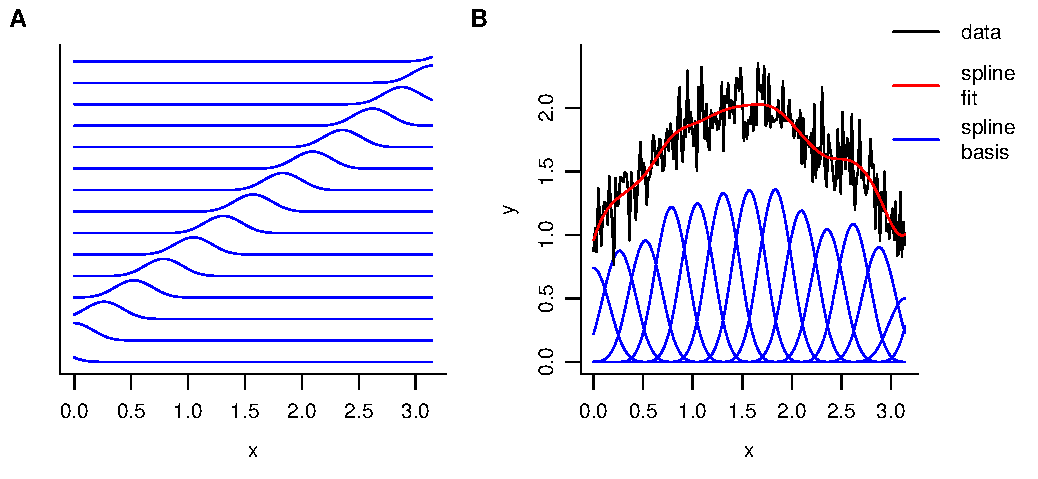
\includegraphics[width=1\textwidth]{fig1.pdf}
    \caption{xxx}
    \label{bspline_regression}
  \end{center}
\end{figure}

A spline is a piecewise function made up of one or more polynomial segments joined together at points known as ``knots''. A wide range of spline functions are possible, however Basis-splines, more commonly known as B-splines, are a popular choice for smoothing applications due to their favorable numerical properties~\cite{DeBoor2001}. The degree of a B-spline function determines its overall smoothness, and third degree (or cubic) B-splines are often used for smoothing. A cubic B-spline basis is show in Figure~\ref{bspline_regression}A with an offset added in the y-direction for clarity. B-spline bases consist of regularly spaced overlapping spline functions, spanning the full range of x values.

A B-spline basis may be used to obtain a smooth estimate of a signal using simple linear regression. Figure~\ref{bspline_regression}B shows the result of a spline regression, where each spline function has been optimally weighted, such that the sum of the functions (spline fit line) is the least squares fit to the data. The desired smoothness of the fit is controlled by adjusting the spline knot spacing, which in turn changes the density of spline functions. In the case of Figure~\ref{bspline_regression}B, 15 functions were found to give a reasonable level of smoothness. Increasing the density of spline functions allows more detail to be captured by the fit, however too many functions results in an increased sensitivity to noise and the smooth estimate begins to exhibit random fluctuations. Conversely, insufficient density of spline functions results in the spline fit being unable to model genuine smooth trends present in the data.

An alternative to adjusting the number of spline basis functions to achieve a desired level of smoothness is to introduce a penalty parameter into to spline regression model. The smooth estimate $\hat{\mathbf{y}}$, of our data $\mathbf{y}$, is calculated as: $\hat{\mathbf{y}} = \mathbf{B} \ \hat{\mathbf{a}}$, where $\mathbf{B}$ is a B-spline basis in matrix form, and $\hat{\mathbf{a}}$ is a vector of corresponding spline weightings to be determined. In simple spline regression $\hat{\mathbf{a}}$ is found by solving the normal equations to minimize the sum of the squared differences between $\mathbf{y}$ and $\hat{\mathbf{y}}$. In penalized spline regression, the minimization function $Q_B$ is adjusted to incorporate an additional term to enforce smoothness in the estimate:

\begin{equation}
  Q_{B} = ||\mathbf{y} - \mathbf{B} \ \hat{\mathbf{a}} ||^{2} + \lambda ||\mathbf{D} \ \hat{\mathbf{a}}||^{2}.
  \label{qb}
\end{equation}

The $\lambda$ parameter controls the degree of smoothness by penalizing solutions for $\hat{\mathbf{a}}$ that interact with the difference matrix $\mathbf{D}$. The difference matrix may be constructed to penalize the first, second or higher orders of differences between the $\hat{\mathbf{a}}$ values. Here, we exclusively use a second order difference matrix, which acts to minimize the second derivative of the smooth estimate.

\begin{equation}
  \mathbf{D} =
  \begin{bmatrix*}[r]
    1 & -2 &  1 &  0 &  0 &  0 & \dots \\
    0 &  1 & -2 &  1 &  0 &  0 & \dots \\
    0 &  0 &  1 & -2 &  1 &  0 & \dots \\
    0 &  0 &  0 &  1 & -2 &  1 & \dots \\
    \vdots & \vdots & \vdots & \vdots & \vdots & \vdots & \ddots \\
  \end{bmatrix*}
  \label{d_mat}
\end{equation}

An example of the second order difference matrix is given in~(\ref{d_mat}), which shows how increased differences between adjacent weighting factors in $\hat{\mathbf{a}}$ consequently increase the penalty term in equation~(\ref{qb}). The minimization function $Q_{B}$ represents a compromise between minimizing the fit residual and smoothness, where a value of zero for $\lambda$ results in simple spline regression. Larger values of $\lambda$ encourage a smoother $\hat{\mathbf{y}}$, to the point where $\hat{\mathbf{y}}$ becomes a straight line fit for very large penalties when using a second order difference matrix. The solution to equation~(\ref{qb}) may be found by augmenting $\mathbf{B}$ and $\mathbf{y}$:

\begin{equation}
  \begin{bmatrix}
    \mathbf{y} \\ 0
  \end{bmatrix}
  \approx
  \begin{bmatrix}
    \mathbf{B} \\ \sqrt{\lambda} \ \mathbf{D}
  \end{bmatrix} \hat{\mathbf{a}} =
  \begin{bmatrix}
    \hat{\mathbf{y}} \\ 0
  \end{bmatrix},
  \label{p-spline_eq}
\end{equation}

and regressing the augmented $\mathbf{y}$ vector on the augmented $\mathbf{B}$ matrix to yield $\hat{\mathbf{a}}$.

The general approach for penalized spline regression is to over-specify the number of B-spline basis functions, and primarily control the smoothness through the adjustment of $\lambda$ acting on a difference matrix. We refer to this approach as ``P-splines'', first introduced by Eilers and Marx~\cite{Eilers1996}. Whilst the value of $\lambda$ has a direct effect on smoothness, it is an unintuitive parameter to interpret as the optimal value often varies by several orders of magnitude. In addition, $\lambda$ has a complex dependence on the density of the spline functions, the number of data points and other factors unrelated to smoothness. A more intuitive measure of the smoothness of a P-spline model is known as the effective dimension (ED), proposed by Hastie and Tibshirani \cite{Hastie1990}. For a given value of $\lambda$, B-spline basis $\mathbf{B}$ and difference matrix $\mathbf{D}$, we calculate ED as follows:

\begin{equation}
  \mathbf{H} =
  \begin{bmatrix}
    \mathbf{B} \\ \sqrt{\lambda}\ \mathbf{D}
  \end{bmatrix}^{-1}
  \begin{bmatrix}
    \mathbf{B} \\ 0
  \end{bmatrix},
\end{equation}

\begin{equation}
  \textrm{ED} = \mathrm{tr}(\mathbf{H}),
\end{equation}

where $\mathbf{H}$ is commonly known as the ``hat'' matrix. For a small value of $\lambda$, ED approaches the number of spline functions in the basis $\mathbf{B}$, and for large values, ED approaches 2 when using a second order difference matrix.

% Figure 2
\begin{figure}
  \begin{center}
    \includegraphics[width=0.9\textwidth]{fig2.pdf}
    \caption{xxx}
    \label{pspline_error}
  \end{center}
\end{figure}

Using simulated data we can investigate the relationship between $\lambda$, ED and the optimal level of smoothness. The top left panel in Figure \ref{pspline_error}A shows a simple sine function with added normally distributed noise, shown in red and black respectively. Candidate P-spline smoothers, with differing values of $\lambda$, are shown in the remaining 5 panels. Since the true shape of the underlying smooth function is known, the error of the P-spline estimate may be calculated and plotted as a function of $\lambda$, shown in Figure \ref{pspline_error}B. The difference between the P-spline estimate and noisy data (residual) and the ED are also shown as a function of $\lambda$ in part B.

% TODO note that error is RSS - is it? what about residual?

Inspection of the error plot reveals the optimal $\lambda$ to be approximately 20 --- corresponding to an ED value of 12, and this can be intuitively verified from part A. For larger values of $\lambda$, the estimate approaches a straight line fit --- failing to capture the details in the sine cure and resulting in an increasing fit residual and fit error (part B). Models with insufficient freedom to adapt to genuine trends in the data result in biased estimates and this is known as ``underfitting''. Conversely, too much freedom in the smoothing model (small $\lambda$) results in the estimate becoming overly sensitive to random fluctuations in the data resulting in ``overfitting''. In least-squares fitting, there is a temptation to equate the smallest residual with the optimal fit, however Figure \ref{pspline_error}B clearly shows an increase in the error for $\lambda$ values of less than 20 --- despite a steady reduction in the residual.

Determining the optimal value for the smoothness parameter is one of the primary challenges for P-spline smoothing. A careful balance between instability from overfitting, and bias from underfitting, must be made for the most accurate estimate, and searching for the smallest fit residual is a useful, but insufficient metric of quality. Numerous approaches have been proposed to find the optimal smoothing value \cite{Ruppert2003}, and in this study we use \textit{Akaike's information criterion} (AIC) \cite{Akaike1973}:

% TODO avoid RSS and talk about y and yhat

\begin{equation}
  \textrm{AIC} = \ln(\textrm{RSS}) + 2 \textrm{ED} / n,
  \label{aic}
\end{equation}

where RSS is the sum of squared differences between the data and smooth estimate, and $n$ is the number of data points. The AIC is typically used to compare models, with lower values indicating an improved balance between bias and instability. A plot of the AIC as a function of $\lambda$ is shown in the lower panel of Figure \ref{pspline_error}B, and the $\lambda$ value with the lowest AIC shows good agreement with the true minimum error.

\subsection{MRS baseline estimation using P-splines}

In $^1\mathrm{H}$ MRS analysis, the baseline signal must be estimated in the presence of numerous overlapping metabolite lipid and macromolecule signals. Fortunately, these non-baseline signals are typically well characterized and may be accurately simulated from known parameters \cite{Govind2015}. We can update Equation \ref{p-spline_eq} to incorporate these additional components by arranging into columns of the matrix $\mathbf{M}$, and appending to the P-spline basis $\mathbf{B}$:

\begin{equation}
  \begin{bmatrix}
    \textbf{y} \\ 0
  \end{bmatrix}
  \approx
  \begin{bmatrix}
    \textbf{B} && \textbf{M} \\ \sqrt{\lambda} \ \textbf{D} && 0
  \end{bmatrix} \hat{\mathbf{a}} =
  \begin{bmatrix}
    \hat{\textbf{y}} \\ 0
  \end{bmatrix},
\end{equation}

As with Equation \ref{p-spline_eq}, we regress the basis matrix on $\mathbf{y}$ to yield $\hat{\mathbf{a}}$, however since metabolite signals are always positive, we can improve analysis stability by enforcing a non-negative constraint on the $\hat{\mathbf{a}}$ values corresponding to the weightings of $\mathbf{M}$. The active-set method developed by Lawson and Hanson \cite{Lawson1995} is used herein to find the least-squares solution under the non-negative constraint --- while still allowing the $\hat{\mathbf{a}}$ values corresponding to the spline basis to remain unconstrained.

% todo table of metabolite names and amplitudes

A simulation study was performed to investigate the relationship between baseline smoothness, the accuracy of metabolite estimates and the AIC. Metabolite signals were simulated from known parameters \cite{Govind2015} at levels consistent with normal brain tissue \cite{deGraaf2018}. A simulated macromolecule profile was also included in the simulation and basis matrix \cite{Birch2017}. Simulated experimental conditions consisted of a field strength of 3T, and semi-LASER localization (TE=28ms). 1024 complex points were generated at a sampling frequency of 2000Hz, 6Hz Gaussian line-broadening was applied prior to zero-filling to 2048 points and Fourier transform to the frequency-domain. Ideal pulses were assumed and relaxation effects were not considered.

Ideal spectra were distorted with normally distributed noise resulting in a spectral SNR of XXXXX. A broad Gaussian resonance was added at 1.3 PPM with a linewidth of 100Hz to simulate baseline distortion originating from scalp lipids. The degree of P-spline baseline flexibility is defined as the baseline ED (effective dimension) per PPM, which is more easily compared across analyses due to its independence from the number of points in the fit and the number of spline basis functions used. Metabolite level estimates were calculated over a range of 10 levels of baseline flexibility, with results averaged across 32 noise realizations at each level to evaluate accuracy and consistency.


% TODO explain how metabolite estimate error and sd was calculated (in terms of a and ahat?)

Metabolite estimation errors are shown in Figure \ref{mrs_bl_simple}A, showing a comparable shape to the simpler model in Figure \ref{pspline_error}B. Over the range of baseline flexibility studied, underfitting with an inflexible baseline results in much greater metabolite estimate errors compared to overfitting --- which can be verified by inspecting the fit result plots in Figure \ref{mrs_bl_simple} parts C-F. Good agreement is also seen between the metabolite estimate error and the AIC curve (part B), with a low AIC values corresponding to the most accurate level of baseline flexibility.

From the results presented in following sections, it was found that the AIC had a tendency to slightly overestimate the optimal level of baseline flexibility and that a simple modification to equation \ref{aic} improved accuracy:

% TODO redefine RSS
\begin{equation}
  \textrm{mAIC} = \ln(\textrm{RSS}) + 2 m \ \textrm{ED} / n.
  \label{maic}
\end{equation}

Setting $m$ to a value of 5 was found to be a good compromise between bias and variance, placing a greater penalty on overly flexible baseline models --- resulting in a smoother ``optimal'' baseline estimate relative to the standard AIC (Figure \ref{mrs_bl_simple}B).

% Figure 3
\begin{figure}
  \begin{center}
    \includegraphics[width=0.9\textwidth]{fig3.pdf}
    \caption{Note the error bars are 5x the true}
    \label{mrs_bl_simple}
  \end{center}
\end{figure}

\subsection{Adaptive Baseline Fitting Algorithm}
In this section we describe a fully-automated $^1\mathrm{H}$ MRS analysis method based on the P-spline fitting approach presented above. The emphasis of the design is to automatically adapt the baseline flexibility for improved accuracy, and we refer to the full algorithm as: \textit{Adaptive Baseline fitting} or ABfit. The algorithm consists of 4 main steps, which will be described in order of execution:

\begin{enumerate}
  \item Coarse frequency alignment.
  \item Approximate iterative fitting.
  \item Baseline smoothness estimation.
  \item Detailed iterative fitting.
\end{enumerate}

\subsubsection{Coarse frequency alignment}
Unprocessed MRS data typically have an unknown and erroneous frequency offset $f_{o}$ that displaces all resonances equally. The first step of ABfit is to estimate $f_{o}$ (measured in Hz) to ensure the basis set of known signals are approximately matched to the acquired data. Raw MRS data is digitally sampled at a frequency of $\mathit{fs}$ Hz in the time-domain, and defined a vector of $N$ complex data points:

\begin{equation}
  \mathbf{y}^{\mathrm{TD}} = \mathbf{y}(\mathbf{t}), \mathbf{t}=(t_{0}=0,t_{1} =1/\mathit{fs},\ldots,t_{N-1}=(N-1)/\mathit{fs}),
\end{equation}

where superscript TD and FD denote time and frequency-domain signal representations --- calculated with the discrete Fourier transform. We simulate a reference data set $\mathbf{r}^{\mathrm{TD}}$, with twice the number of data points $2N$ sampled at $\mathit{fs}$, containing three resonances corresponding to the main singlet metabolites typically present in $^1\mathrm{H}$ MRS data at 2.01, 3.03 and 3.22 PPM. The acquired data $\mathbf{y}^{\mathrm{TD}}$ is zero-filled to twice the original length --- before convolving with  $\mathbf{r}^{\mathrm{TD}}$ to estimate the frequency offset $f_{o}$.

% TODO check above is correct - surely the FD versions (not TD) of y and r are convolved?

\subsubsection{Approximate iterative fitting}
The goal of this stage of the algorithm is to find estimates of the three parameters with the largest influence on the fit residual: 1) the signal phase $\phi_{0}$; 2) an approximate lineshape parameter $d_{g}$ and 3) an improved estimate of $f_{o}$. The phase and frequency offset are applied to the acquired data as follows:

\begin{equation}
  \mathbf{y'}^{\mathrm{TD}} = \mathbf{y}^{\mathrm{TD}} e^{i \phi_{0} + 2 i \pi f_{o} \mathbf{t}}
\end{equation}

where the phase parameter $\phi_{0}$ is measured in radians and $i=\sqrt{-1}$. The lineshape parameter applies Gaussian line-broadening to each signal in the basis set $\mathbf{M}$:

\begin{equation}
  \mathbf{M}'^{\mathrm{TD}} = \mathbf{M}^{\mathrm{TD}} \star e^{-d_{g}\mathbf{t}^{2}}
\end{equation}

where $\star$ denotes element-wise multiplication of the line-broadening function for each column of the basis matrix. Combining the modified basis with the P-spline basis and solving for $\hat{\mathbf{a}}$ in the least-squares sense with the same constraints as the previous section:

\begin{equation}
  \begin{bmatrix}
    \textbf{y}'^{\mathrm{FD}}_{s} \\ 0
  \end{bmatrix}
  \approx
  \begin{bmatrix}
    \textbf{B} && \textbf{M}'^{\mathrm{FD}}_{s} \\ \sqrt{\lambda} \ \textbf{D} && 0
  \end{bmatrix} \hat{\mathbf{a}} =
  \begin{bmatrix}
    \hat{\textbf{y}} \\ 0
  \end{bmatrix}.
\end{equation}

Note that following parametric modification in the time-domain, the data and basis of known signals are zero-filled to twice their original length before being transformed to the frequency-domain. Only the real valued data points in frequency domain between 1.9 and 4 PPM are fit in this stage of the algorithm (denoted by subscript $s$) to reduce the influence of any contaminating lipid signals around 1.3 PPM. The parameters: $\phi_{0}$, $d_{g}$ and $f_{o}$ are estimated using Nelder-Mead simplex algorithm with bound constraints \cite{Box1965}, minimizing:

\begin{equation}
  || \textbf{y}'^{\mathrm{FD}}_{s}  - \hat{\textbf{y}} ||^{2}.
\end{equation}

A $\lambda$ value corresponding to 1 ED per PPM is used with a P-spline basis with 15 components per PPM. Constraints placed on the optimization algorithm restrict the linebroading parameter to be positive and produce a lineshape of less than 15 Hz FWHM, additionally the frequency offset must be less than 10 Hz different from the coarse frequency alignment step.

\subsubsection{Baseline smoothness estimation}
Following the determination of the frequency offset, spectral phase and approximate lineshape the next step of ABfit is to estimate the optimal value for $\lambda$. A set of candidate fits are performed with differing level of baseline smoothness, whilst maintaining the three main fitting parameters constant at their optimized values. The maximum candidate baseline flexibility is set to a $\lambda$ value corresponding to 7 ED per PPM, and the minimum value set to an ED of 2 --- equivalent to straight line fit. 15 candidate fits are performed with logarithmic intervals between the maximum and minimum values, and the mAIC is calculated for each fit (Equation \ref{maic}). The optimal $\lambda$ value is chosen as the value used for the candidate fit with the lowest mAIC. In contrast to the previous step, a wider spectral range of 0.2 to 4 PPM is analyzed to include the majority of conventionally measured metabolites.

\subsubsection{Detailed iterative fitting}
In the final stage of ABfit, the overall lineshape model is refined alongside minor adjustments to the frequencies and linewidths of the known basis signals.

\cite{Stancik2008}

\subsection{Simulation validation}

\subsection{MRSI data validation}

\section{Results}
XXXX

\section{Discussion}
MRM open science paper: https://onlinelibrary.wiley.com/doi/full/10.1002/mrm.27939

\cite{Stikov2019}

% compare with LCModel P-spline approach which is more like O'Sullivan1986.

\cite{OSullivan1986}

% comment on following paper : Regularized semiparametric model identification with application to nuclear magnetic resonance signal quantification with unknown macromolecular base‐line.

% Comment on Brian S's paper

\section{Conclusion}
XXXX

\section*{ACKNOWLEDGEMENTS}
XXXX

\bibliography{main}

\clearpage
\listoffigures

\end{document}

%%% Local Variables:
%%% ispell-local-dictionary: "american"
%%% End:
